%
% File main.tex
%
% Contact: car@ir.hit.edu.cn, gdzhou@suda.edu.cn
%%e.agirre@ehu.es or Sergi.Balari@uab.es
%% and that of ACL 08 by Joakim Nivre and Noah Smith

\documentclass[11pt]{article}
\usepackage{acl2015}
\usepackage{times}
\usepackage{url}
\usepackage{latexsym}
\usepackage{graphicx}



\makeatletter
\newcommand{\@BIBLABEL}{\@emptybiblabel}
\newcommand{\@emptybiblabel}[1]{}
\makeatother
\usepackage{hyperref}

%\setlength\titlebox{5cm}

% You can expand the title box if you need extra space
% to show all the authors. Please do not make the title box
% smaller than 5cm (the original size); we will check this
% in the camera-ready version and ask you to change it back.


\title{Spoiler detection and extraction\\Project Proposal for NLP Course, Winter 2022}

\author{M. Kierznowski, Ł. Pancer, P. Wesołowski \\
  Warsaw University of Technology \\
%   {\tt email@domain} \\
  \And
    supervisor: Anna Wróblewska \\
  Warsaw University of Technology \\
    {\tt anna.wroblewska1@pw.edu.pl}
    }

\date{}

\begin{document}
\maketitle
\begin{abstract}
In this document, we present a literature review, describe project ideas and provide an initial outline of the solution for the first NLP course project. The project will address the spoiler detection task. Current research in this field mainly relates to classification without touching the model interpretability. The main goal is to create a novel benchmark for evaluating the performance of the spoiler classification. The benchmark would analyze the model's rationale and compare it with precise human knowledge. We are going to evaluate the performance of the state-of-the-art models with our tool. Besides, we are going to extend the previous spoiler detection works by utilizing a new dataset, hoping for an improvement in performance.

%   Write about the proposed work touching the research gap you are addressing, novelty, and on the proposed deliverable aimed from this project.  
%   (Short description up to 250 words.)
\end{abstract}

\section{Introduction}
In everyday life, information that reveals the important aspects, events, and twists of a plot of, e.g., a book, a movie, or a videogame is referred to as a spoiler. Spoilers are usually undesired, and getting to know one of them may contribute to a decrease in enjoyment \cite{abbott2020can} or a lack of further interest in reading or seeing the particular position \cite{li2022exploring}. However, they can often become known by chance, for example, due to being a part of some review. Therefore, automatic spoiler detection has become one of the crucial tasks in the NLP field \cite{guo2010finding}.

Several methods on this issue have been proposed. While the authors often focus on their classification performance, we believe that the interpretability aspects are also important and may be an adequate measure of the actual performance. Therefore we are going to develop a tool for the assessment of the spoiler classification performance on the basis of the model rationale.

The use of transfer learning has already become pretty standard due to better performance, reduction of training time, electricity usage, etc. However, proper fine-tuning on the task-related dataset may be important for further improvement in the model's robustness and accuracy. Similarly to our predecessors, we are going to utilize powerful pre-trained models. However, we would like additionally to make use of the IMDB reviews dataset \cite{enam_biswas_2021}, which does not appear to be frequently used. We believe that due to its size (and, therefore, probably its diversity), it may be a good source of additional knowledge for our models.

Our project is driven mainly by two questions: 
\begin{enumerate}
    \item How do the numeric measurements of the model performance (accuracy, recall, etc.) relate to its performance evaluated in a more strict but interpretability-based way?
    \item Does providing a larger task-related dataset for fine-tuning result in the improvement of the spoiler detection model?
\end{enumerate}

\section{Literature Review} \label{literature-review}

Spoiler detection tasks had been previously neglected, and only in recent years it saw more rapid development. Early studies related to spoiler detection treated it as a traditional classification task, most commonly utilizing methods such as Support Vector Machines. The progress revolved around the process of building a larger dataset with more linguistic features available. Publications explored basic Bag-of-Words approaches: creating a blacklist of words for a given topic \cite{golbeck2012twitter}, introducing temporal filtering system \cite{nakamura2007temporal}, using topic models based on Latent Dirichlet Allocation \cite{guo2010finding}. Significant contributions to publicly available datasets include TV Tropes Movies \cite{boyd2013spoiler} and GoodReads dataset \cite{wan2019fine}. Chang \shortcite{chang2018deep} proposed an attention-based solution, and today similar approaches still remain state-of-the-art. More recently, a transfer learning approach was suggested, laying the stress on interpretability \cite{wroblewska2021spoiler}. On the topic of interpretability, publications of LIME \cite{lime}, and SHAP \cite{NIPS2017_7062} are particularly interesting. LIME is an explanation technique designed to explain black-box models, which are common in the NLP field due to the high-dimensional nature of features. It uses a local linear approximation to explain the model's predictions. SHAP is a superset of LIME, basing the explanations on a game theory concept of Shapley values. LIME and SHAP in NLP models allow extract words that are responsible for making a certain prediction and provide metrics on the strength of their contribution. DeYoung \shortcite{deyoung2019eraser} introduced a benchmark based on datasets with rationales annotated by humans to assess the interpretability of NLP models by comparing their rationales with humans'.


\section{State of the Art}
The provided literature, as well as other state-of-the-art solutions, are based upon a Bidirectional Encoder Representations from Transformers (BERT) architecture \cite{devlin2018bert}. BERT is an eminently versatile solution, finding use in many corners of the Natural Language Processing field. It was originally developed at Google AI Language and includes the encoder part of the transformer architecture to create word embeddings. Figure 1 shows the bidirectional nature of the encoder. A sequence of words is processed at once, making it possible to extract the context of a word from both the preceding as well as following words.
\begin{figure}[h]
\begin{center}
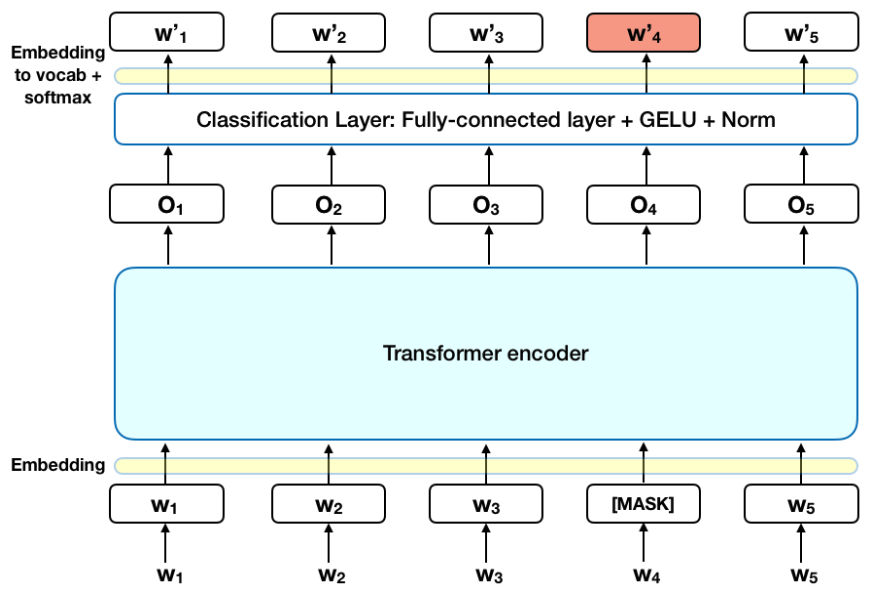
\includegraphics[width=0.45\textwidth]{Bert.png}
\caption[]{BERT Architecture Diagram}
\url{https://miro.medium.com/max/1400/0*ViwaI3Vvbnd-CJSQ.webp}
\label{bert_arch}
\end{center}
\end{figure}


GloVe (Global Vectors) \cite{pennington2014glove} is another popular algorithm for creating word embeddings. It makes use of a word co-occurrence counts matrix to calculate a conditional probability of words being present in a given context, which is used as a measure of semantic similarity. The words are arranged in the vector space to connect the distance between words to similarity. The adoption of word co-occurrence allows extracting global as opposed to only local relationships between words. However, an inevitable disadvantage of GloVe is the inability to differentiate homographs, i.e., words that are spelled the same but have a different meaning.


\section{General outline}
To our knowledge, the current research on spoiler detection task mainly concerns classification, and the performance is assessed using widely known quantitative metrics. Still, there exist datasets, mentioned in section \ref{literature-review}, with annotated spoiler phrases (with a sentence- or word-level annotations). We would like to investigate whether the machine learning models developed for the classification of the whole documents, viz. containing a spoiler or not, actually correctly identify these phrases. More strictly, we would like to know if the annotated document phrases are effectively responsible for classifying a review as a spoiler.

We would like to focus on the assessment of the document classification in the following way. For every document classified as containing a spoiler, we want to use XAI tools to get the phrases that determined the model decision. Then, we can compare the crucial set of phrases with the ones selected by annotators (either word- or sentence-level). The comparison can be made using different metrics. As for now, we consider Jaccard's similarity.

Going into the details, in our work, we are going to use the following datasets:
\begin{itemize}
    \item Goodreads - 1.3M documents, 17M sentences, 570k spoiler sentences,
    \item TV Tropes Books - 340k documents, 670k sentences, 110k spoiler sentences,
    \item IMDB reviews - 5.5M documents, 1.1M spoiler documents.
\end{itemize}

The first dataset consists of reviews with spoiler fragments annotated by the community. Goodreads members can mark text using introduced spoiler tags in order to hide specific phrases. We are going to create a balanced version of this dataset, as it was done by Wróblewska \shortcite{wroblewska2021spoiler}. The TV Tropes Books dataset provides word-level annotations hence it's the most valuable for us. The IMDB reviews dataset offers only document-level annotations.

Regarding the models used, we would probably utilize the ones used in similar works. We are going to use deep learning models built on top of pre-trained state-of-the-art solutions. However, we would like to fine-tune the models first using IMDB dataset. We would like to know if such a procedure is helpful for the task considered.


% Detailed description (up to 12 pages) in English, including the following information:
% \begin{enumerate}
% \item the scientific goal of the project (description of the problem to be solved, research questions and hypotheses);
% \item significance of the project (state of the art, justification for tackling a specific scientific problem, justification for the pioneering nature of the project, the impact of the project results on the development of the research field and scientific discipline);
% \item concept and work plan (general work plan - with a timeline, specific research goals, results of preliminary research, risk analysis);
% \item approach \& research methodology (underlying scientific methodology, methods, techniques and research tools, methods of results analysis, equipment and devices to be used in research);
% \item well-justified project literature (a reference list for publications included in the project description, with full bibliographic data).
% \end{enumerate}

\section{Concept and Work Plan}
Regarding topic our plan is to conduct a research on detecting spoilers using state-of-the-art architectures like BERT or RoBERTa. Subsequently we want to use various XAI techniques in order to understand with words model consist to be spoilers. Going into the details we want to test Local Interpretable Model-agnostic Explanations (LIME) which perturbs instance we want to explain, learns a sparse linear model around it, as an explanation \cite{ribeiro2016should}.
For the next XAI method  Evaluating Rationales And Simple English Reasoning (ERASER) which is benchmark to advance research
on interpretable models in NLP. Furthermore attention layers is another candidate for incorporating XAI method in work. However we need to remember that not all languages models has it's own attention layers to work with. The goal of final analysis is to develop end-to-end architecture that properly distinguish spoilers reviews and provide information why specific words triggers model (and with what strength). However introduced approaches may be connected with some risk factors. Firstly not all language models will equally response for XAI techniques e.g previously mentioned attention layer. Subsequent issue may concern data sets which are build differently concerning annotation level. TV Tropes Books has every word-level annotation whereas Goodreads only sentence-level and  IMDB only document annotations. It may lead to abandonment of some source of data e.g ERASER needs to have word-level annotations.



\section{Summary}
In this document, we described our preliminary findings pertaining to the first NLP course project. We believe that any interesting conclusions and observations may lead to more interpretability-oriented research in the future. We expect that analyzing the quality of a model not only based on hard measures but also on consistency with human annotators can lead to better solutions. In particular, we hope that it has the chance to help in the further advances of automatic spoiler detection, which from our perspective, is an important subject.

% include your bib file like this:
\bibliographystyle{acl}
\bibliography{bibliography}

\end{document}